\chapter{Despliegue}
    En este capítulo se detalla cómo, una vez terminada una versión funcional de la aplicación, se comienza con el proceso de habilitar el uso de la aplicación desde la web. Para ello decidimos utilizar la plataforma Hostinger\cite{hostinger}, y todos los servicios que la misma proporciona a sus usuarios.
    \newline
    
    Elegimos Hostinger y no otras alternativas como Microsoft Azure\cite{azure} debido a ciertas características que lo hacían diferente de los demás. Por una parte Hostinger posee un sistema de  configuración fácil, tanto para el lado \textit{backend} como el \textit{frontend} y para la gestión de las bases de datos relacionales mediante phpMyAdmin. Otra razón de peso es que este servicio de \textit{hosting} posee un chat en español disponible 24 horas al día durante todo el año, de esta manera ante cualquier imprevisto contamos con la ayuda de los mismos. \newline
    
    El despliegue de la aplicación consta de tres partes; el despliegue de la aplicación \textit{frontend}, el despliegue de la aplicación \textit{backend}, y el despliegue de la base de datos.
    
    \section{Frontend}
    Para desplegar la aplicación Angular que representa el \textit{frontend} de nuestra aplicación, se utilizó la herramienta ``Administrador de archivos'' que nos ofrece Hostinger y que nos proporciona una interfaz de usuario para administrar archivos y directorios en nuestro dominio \textit{tfg-estudio-medico.com}.
    \newline
    
    En dicho administrador, se procedió a subir la carpeta \textit{dist} generada por el proyecto Angular.
    
     \begin{figure}[h]
    \centering
     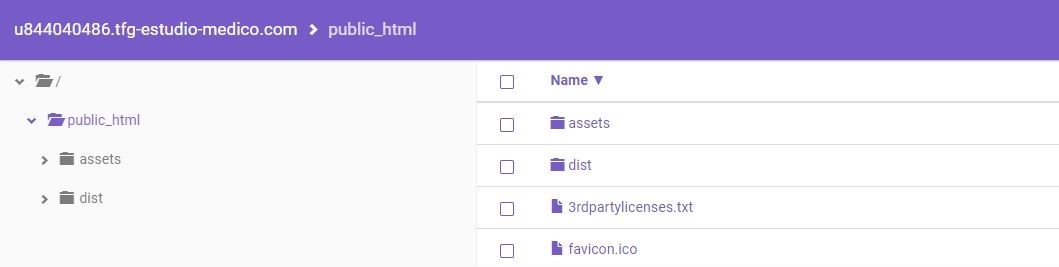
\includegraphics[width=1\textwidth]{images/administradorarchivos3.jpg}
    \caption{Administrador de archivos de Hostinger}
    \end{figure}
    

    \section{Backend}
    Para desplegar la aplicación Java Spring que constituye el \textit{backend} de nuestra aplicación, se utilizó un servidor proporcionado por Hostinger\cite{hostinger}. En dicho servidor instalamos un sistema operativo Ubuntu 18.04 64bit.
    
     \begin{figure}[h]
    \centering
     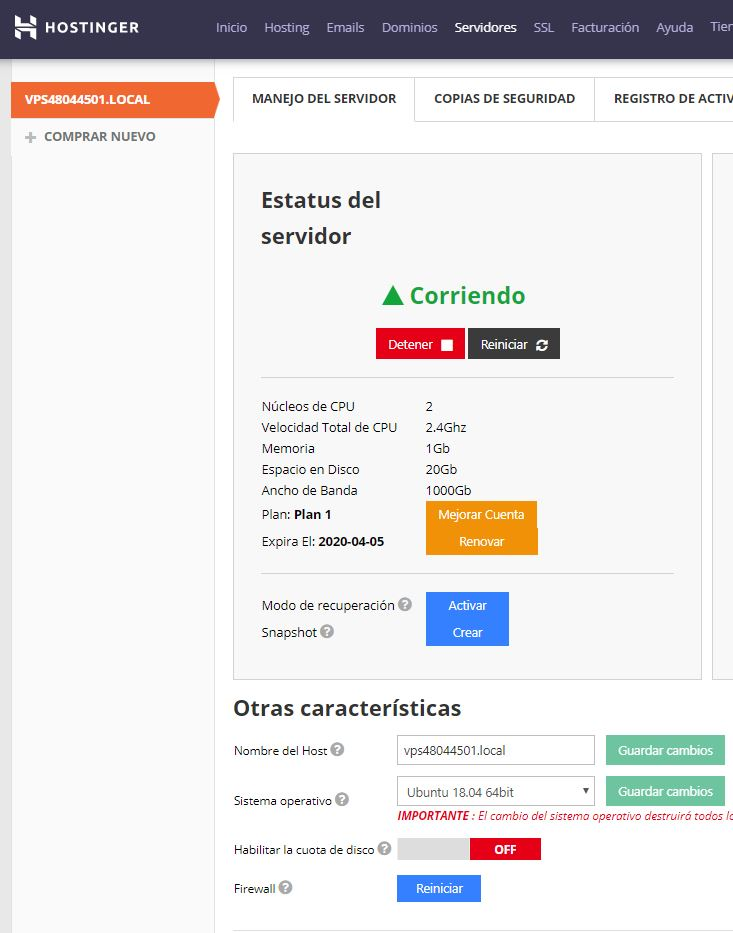
\includegraphics[width=0.9\textwidth]{images/servidorhostinger}
    \caption{Servidor en Hostinger}
    \end{figure}
    
    \FloatBarrier
    
    Para conectarnos al servidor utilizamos el programa MobaXterm, conectándonos al servidor a traves de SSH. Nuestro objetivo era mantener el archivo .jar ejecutándose en la máquina incluso si no estamos conectados a la misma, para ello generamos un \textit{servicio}, esto es, un script que se mantiene arrancado incluso si cerramos la sesión. \\
    \newline
    Lo primero que tenemos que hacer es generar el archivo ejecutable de nuestro proyecto \textit{backend}. Una vez generado el archivo SNAPSHOT .jar de nuestro proyecto Java Spring, nos disponemos a subirlo a la carpeta /root/back.
    
    \begin{figure}[h]
    \centering
     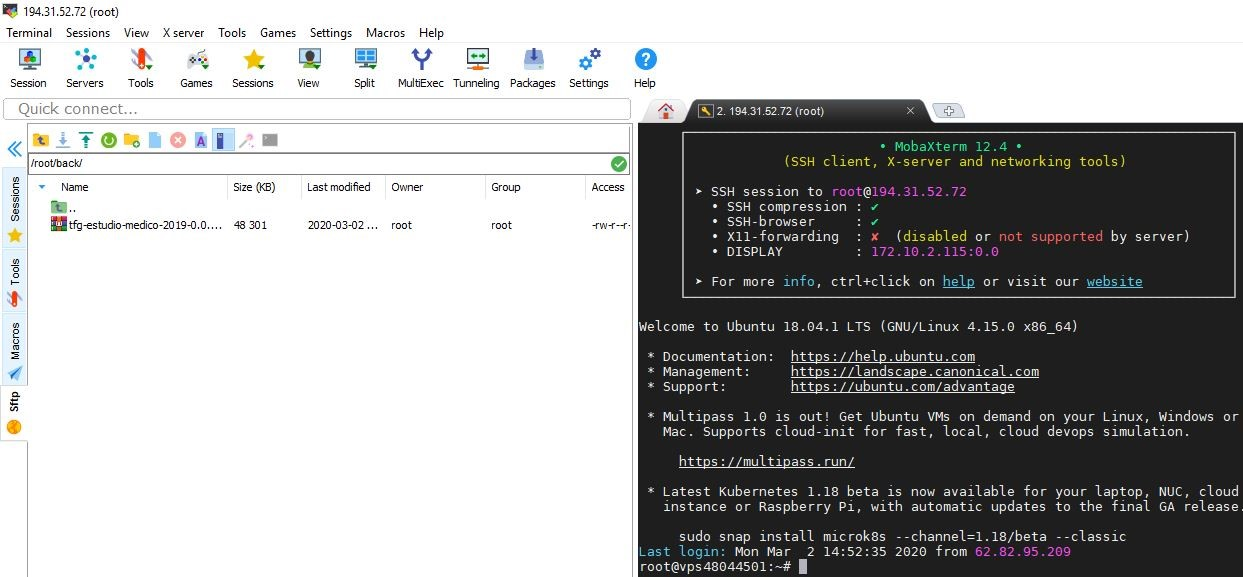
\includegraphics[width=1\textwidth]{images/jarback2.jpg}
    \caption{Jar desplegado en MobaXterm}
    \end{figure}
    
     \FloatBarrier
    
    A continuación, generamos un script llamado \textit{start\_back.sh}  que simplemente ejecuta el comando \textit{java -jar} para arrancar el ejecutable .jar, el cual vamos a guardar en el directorio /usr/local/bin. Lo guardamos en dicho directorio debido a que este directorio es accesible por todos los usuarios.
    
    \begin{figure}[h]
    \centering
     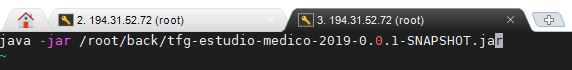
\includegraphics[width=1\textwidth]{images/script}
    \caption{Script start\_back.sh desplegado en MobaXterm}
    \end{figure}
    
     \FloatBarrier
    
    Después hemos generado un \textit{servicio} llamado \textit{daemonback.service} en la carpeta /etc/systemd/system, que es el directorio indicado en sistemas Linux para almacenar y gestionar demonios. Este servicio se encarga de ejecutar en segundo plano el script \textit{start\_back.sh}. 
    
    \begin{figure}[h]
    \centering
     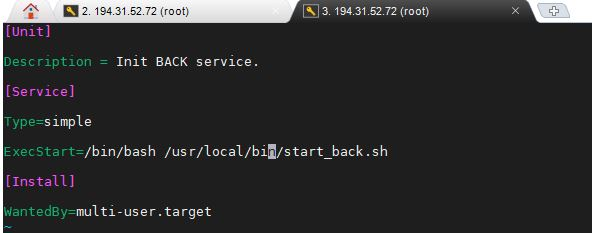
\includegraphics[width=1\textwidth]{images/demonio}
    \caption{Servicio daemonback.service desplegado en MobaXterm}
    \end{figure}
    
     \FloatBarrier
    
    Por último, tan solo tenemos que ejecutar el servicio generado previamente con el comando \texttt{sudo service daemonback start}. Para ver el estado del .jar, ejecutamos el comando \texttt{sudo service daemonback status} y nos muestra lo siguiente:
    
    \begin{figure}[h]
    \centering
     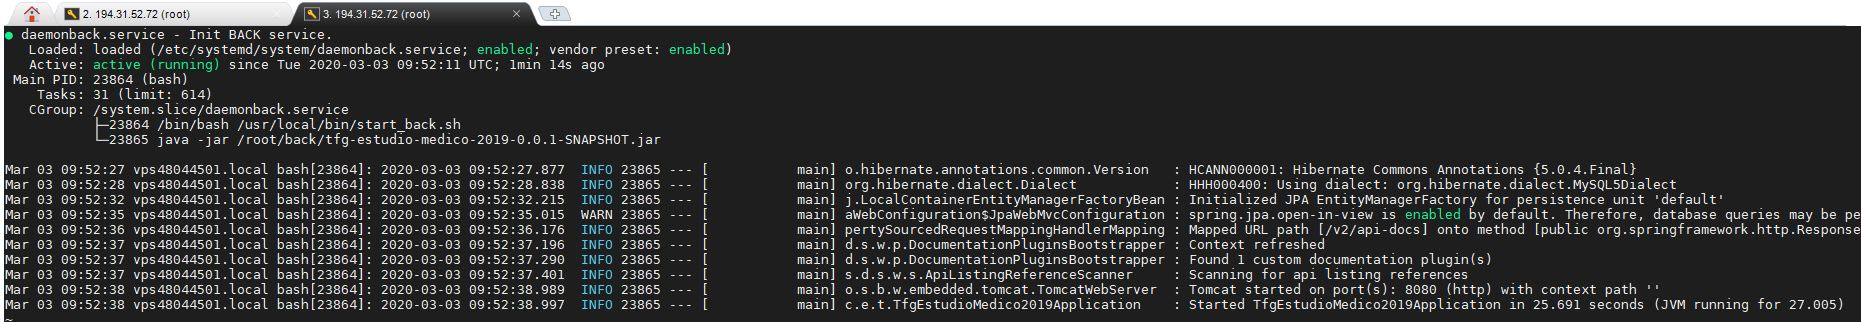
\includegraphics[width=1\textwidth]{images/serviciostart}
    \caption{Estado servicio}
    \end{figure}
    
    
    


    
    \section{Base de Datos}
    Para desplegar la base de datos en la web, se utilizó un servicio que ofrece Hostinger para desplegar bases de datos MySQL. 
    \newline 
    A través de PhpMyAdmin y con la opción de generar la base de datos automáticamente al ejecutar un proyecto Java Spring con JPA, se generó la siguiente base de datos:
    
     \begin{figure}[h]
    \centering
     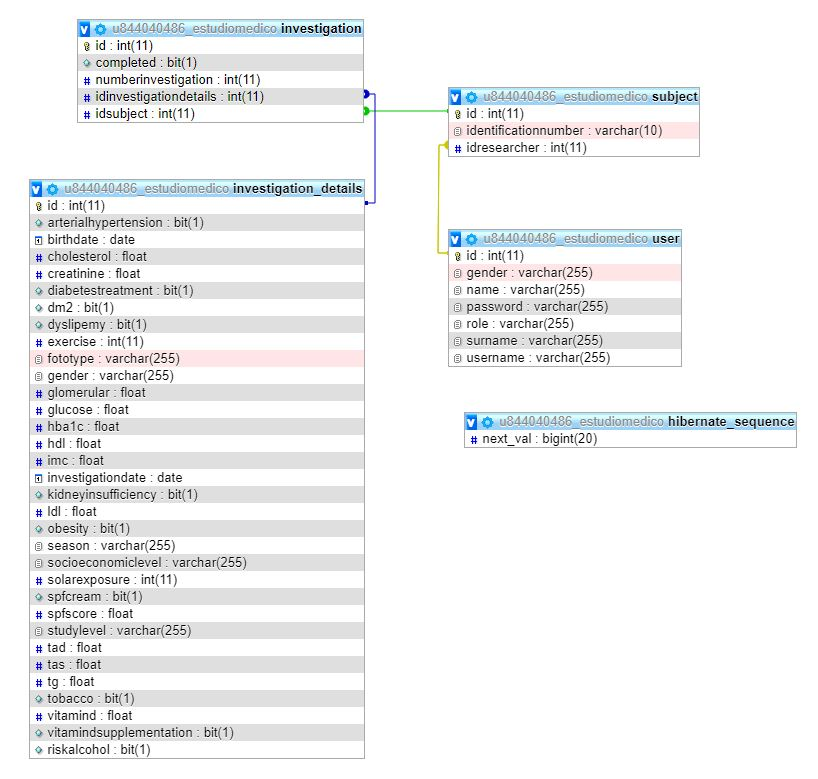
\includegraphics[width=1\textwidth]{images/modelodatos}
    \caption{Modelo de datos generado en PhpMyAdmin}
    \end{figure}
    
    
